%%%%%%%%%%%%%%%%%%%%%%%%%%%%%%%%%%%%%%%%%%%%%%%%%%%%%%%%%%%%%%%%%%%%%%
% LaTeX Example: Project Report
%
% Source: http://www.howtotex.com
%
% Feel free to distribute this example, but please keep the referral
% to howtotex.com
% Date: March 2011 
% 
%%%%%%%%%%%%%%%%%%%%%%%%%%%%%%%%%%%%%%%%%%%%%%%%%%%%%%%%%%%%%%%%%%%%%%
% How to use writeLaTeX: 
%
% You edit the source code here on the left, and the preview on the
% right shows you the result within a few seconds.
%
% Bookmark this page and share the URL with your co-authors. They can
% edit at the same time!
%
% You can upload figures, bibliographies, custom classes and
% styles using the files menu.
%
% If you're new to LaTeX, the wikibook is a great place to start:
% http://en.wikibooks.org/wiki/LaTeX
%
%%%%%%%%%%%%%%%%%%%%%%%%%%%%%%%%%%%%%%%%%%%%%%%%%%%%%%%%%%%%%%%%%%%%%%
% Edit the title below to update the display in My Documents
%\title{Project Report}
%
%%% Preamble
\documentclass[paper=a4, fontsize=11pt]{scrartcl}
\usepackage[T1]{fontenc}

\usepackage[english]{babel}	% English language/hyphenation
\usepackage[protrusion=true,expansion=true]{microtype}	
\usepackage{amsmath,amsfonts,amsthm} % Math packages
\usepackage[pdftex]{graphicx}
\usepackage{array} % allow the parameter 'm' to be used in tabular
\usepackage{placeins} % defines the \FloatBarrier command

%%% Custom sectioning
\usepackage{sectsty}
\allsectionsfont{\centering \normalfont\scshape}

% Define graphics path
\graphicspath{{figs/}}

% increase table height factor a little bit (taller cells)
\renewcommand{\arraystretch}{1.5}

%%% Custom headers/footers (fancyhdr package)
\usepackage{fancyhdr}
\pagestyle{fancyplain}
\fancyhead{}											% No page header
\fancyfoot[L]{}											% Empty 
\fancyfoot[C]{}											% Empty
\fancyfoot[R]{\thepage}									% Pagenumbering
\renewcommand{\headrulewidth}{0pt}			% Remove header underlines
\renewcommand{\footrulewidth}{0pt}				% Remove footer underlines
\setlength{\headheight}{13.6pt}


%%% Equation and float numbering
\numberwithin{figure}{section}			% Figurenumbering: section.fig#
\numberwithin{table}{section}			% Tablenumbering: section.tab#

%%% Maketitle metadata
\newcommand{\horrule}[1]{\rule{\linewidth}{#1}} 	% Horizontal rule

\title{
		%\vspace{-1in} 	
		\usefont{OT1}{bch}{b}{n}
		\normalfont \normalsize \textsc{Diagnostics Group - Brazilian Synchrotron Light Laboratory} \\ [25pt]
		\horrule{0.5pt} \\[0.4cm]
		\huge Custom cable for DMM7510-BCM digital I/O \\
		\horrule{2pt} \\[0.5cm]
}
\author{
		\normalfont 								\normalsize
%        Firstname Lastname\\[-3pt]		\normalsize
        \today
}
\date{}


%%% Begin document
\begin{document}
\maketitle
\section{DMM7510-BCM digital I/O cable}
The DMM7510 multimeter digital I/Os are used to control the BCM functions remotely. Both devices use DB9 connectors for digital I/O. This document describes the pinout of both devices DB9 connectors and how pins on both ends of the connecting cable map to each other.

% Instrument Setup figure
\begin{figure}[!h]
	\caption{DB9 connector pinout}
	\label{fig:db9-pins}
	\centering
	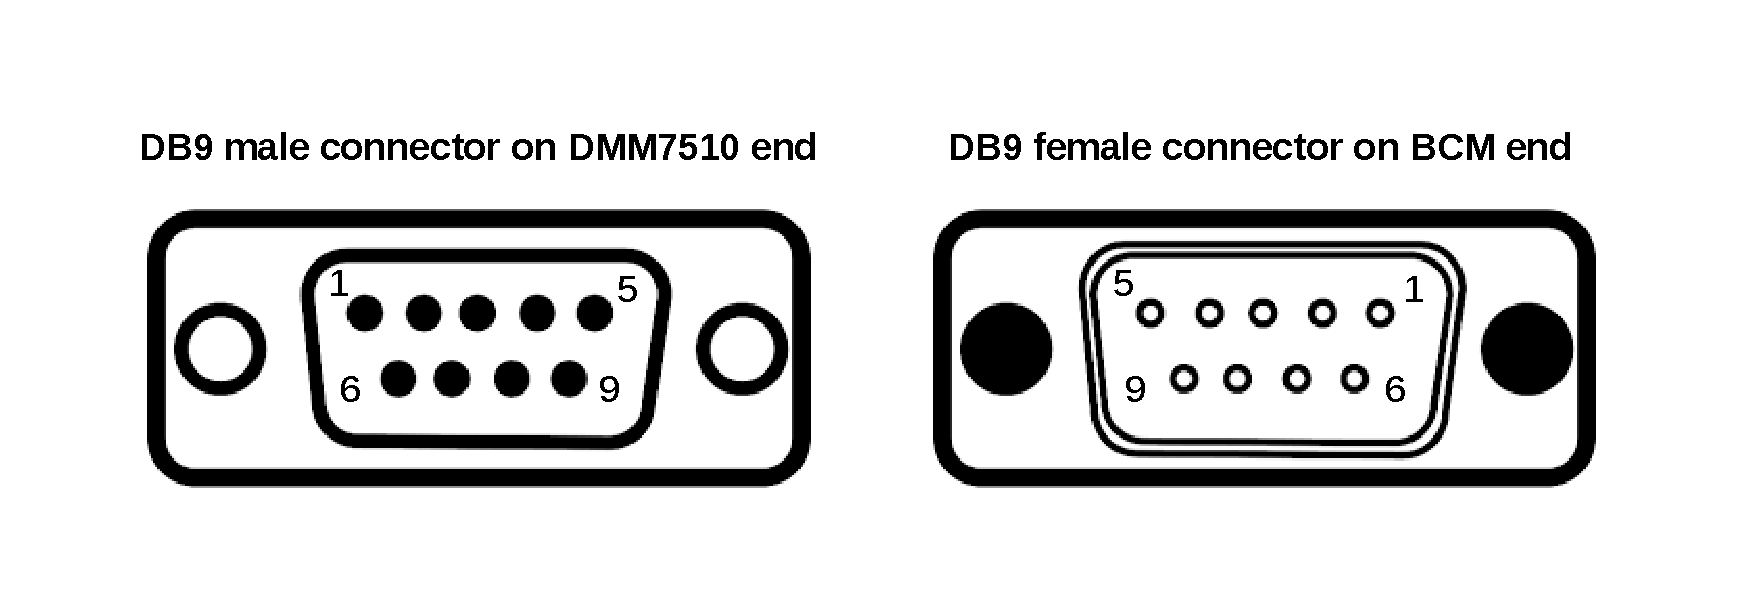
\includegraphics[width=1.0\textwidth]{bcm_db9_connectors}
\end{figure}
\FloatBarrier

\begin{table}
	\center
	\caption{BCM DB9 Pinout}
	\begin{tabular}{m{8cm} m{2cm}}
		\bfseries BCM Function & \bfseries BCM DB9 Pin \\ \hline
		Range selection Bit-2 (MSB) & 3 \\ \hline
		Range selection Bit-1 & 8 \\ \hline
		Range selection Bit-0 (LSB) & 4 \\ \hline
		Calibration enable & 5 \\ \hline
		Calibration charge selection Bit-1 (MSB) & 1 \\ \hline
		Calibration charge selection Bit-0 (LSB) & 6 \\ \hline
		GND & 9 \\ \hline
		Calibration polarity [NOT USED] & 2 \\ \hline
		Output polarity [NOT USED] & 7 \\ \hline
	\end{tabular}
\end{table}

\begin{table}
	\center
	\caption{DMM7510 DB9 Pinout}
	\begin{tabular}{m{8cm} m{2cm}}
		\bfseries DMM7510 Function & \bfseries DMM7510 DB9 Pin \\ \hline
		Line 1 & 1 \\ \hline
		Line 2 & 2 \\ \hline
		Line 3 & 3 \\ \hline
		Line 4 & 4 \\ \hline
		Line 5 & 6 \\ \hline
		Line 6 & 8 \\ \hline
		GND & 9 \\ \hline
		+5 V [NOT USED] & 7 \\ \hline
		Relay flyback [NOT USED] & 5 \\ \hline
	\end{tabular}
\end{table}

\begin{table}
	\center
	\caption{DMM7510-BCM DB9 connections mapping}
	\begin{tabular}{m{2cm} m{2cm} m{4cm} m{6cm}}
		\bfseries DMM7510 DB9 Pin & \bfseries BCM DB9 Pin & \bfseries DMM7510 Function & \bfseries BCM Function \\ \hline
		1 & 1 & Line 1 & Cal. charge selection bit-1 \\ \hline
		2 & 5 & Line 2 & Cal. enable \\ \hline
		3 & 3 & Line 3 & Range selection bit-2 \\ \hline
		4 & 4 & Line 4 & Range selection bit-0 \\ \hline
		5 & - & - & - \\ \hline
		6 & 6 & Line 5 & Cal. charge selection bit-0 \\ \hline
		7 & - & - & - \\ \hline
		8 & 8 & Line 6 & Range selection bit-1 \\ \hline
		9 & 9 & GND & GND \\ \hline
	\end{tabular}
\end{table}

%%% End document
\end{document}
